\documentclass[lettersize,journal]{IEEEtran}

%%%%%%%%%%%%%%%%%%%%%%%%%%%%%%%%%%%%%%%%%%%%%%%%%%%%%%%%%%%%%
% 							HEADER
%%%%%%%%%%%%%%%%%%%%%%%%%%%%%%%%%%%%%%%%%%%%%%%%%%%%%%%%%%%%%

\IEEEoverridecommandlockouts
% The preceding line is only needed to identify funding in the first footnote. If that is unneeded, please comment it out.
\usepackage{amsmath,amssymb,amsfonts}
%\usepackage{cite}
\newcommand{\je}[1]{\textcolor{blue}{#1}}

\usepackage{algorithm}
\usepackage{algpseudocode}
\usepackage{graphicx}
\graphicspath{{./Figures/}} % folder for graphs
\usepackage{float}
%\usepackage{subfigure}
\usepackage[font=footnotesize, justification=justified, singlelinecheck=false]{caption}
%\usepackage[caption=false,font=normalsize,labelfont=sf,textfont=sf]{subfig}
\usepackage{subcaption}
\usepackage{textcomp}
\usepackage[table,xcdraw]{xcolor}
\def\BibTeX{{\rm B\kern-.05em{\sc i\kern-.025em b}\kern-.08em
    T\kern-.1667em\lower.7ex\hbox{E}\kern-.125emX}}

\makeatletter
\newcommand{\linebreakand}{%
\end{@IEEEauthorhalign}
\hfill\mbox{}\par
\mbox{}\hfill\begin{@IEEEauthorhalign}
}
\makeatother

\usepackage{array}
\newcolumntype{P}[1]{>{\centering\arraybackslash}p{#1}}

\setlength{\arrayrulewidth}{0.2mm}
\setlength{\tabcolsep}{2pt}
\renewcommand{\arraystretch}{1.4}
\usepackage{tabularray}
	
\usepackage{tikz,color}
\usepackage{smartdiagram}
\usepackage{cuted}
\usepackage{multirow}

\usepackage[babel]{csquotes}
\usepackage[backend=biber,style=ieee, style=numeric-comp]{biblatex}
\DeclareLanguageMapping{spanish}{spanish-apa}
\addbibresource{Bibliography.bib}

\renewcommand*{\bibfont}{\footnotesize}

\usepackage{tikz}
\usetikzlibrary{shapes,arrows.meta,calc,positioning}
\usepackage{pgfplots}	
\usetikzlibrary{shapes.arrows}%
\usetikzlibrary{shapes.symbols}

\begin{document}
	\title{Semantically-Structured Multimodal 3D Descriptor Learning for Urban Place Recognition}

\author{
        \IEEEauthorblockN{Alvaro Navarro-Perez,
                      Bladimir Bacca-Cortes,
                      Eduardo Caicedo-Bravo}

        \thanks{The associate editor coordinating the review of this manuscript and approv-ing it for publication was Bladimir Bacca (Corresponding author: Alvaro Navarro-Perez)}

        \thanks{Alvaro Navarro-Perez is with Faculty of Engineering, Electronic Engineering, Technologycal Development Research Group (GIDET), Universidad del Quindío, Armenia, Colombia. (email: aanavarro@uniquindio.edu.co)} 

        \thanks{Bladimir Bacca-Cortes is with School of Electrical Engineering, Perception and Intelligent Group, (PSI), Universidad del Valle, Cali, Colombia: (email: bladimir.bacca@correounivalle.edu.co) }

        \thanks{Eduardo Caicedo-Bravo is with School of Electrical Engineering, Perception and Intelligent Group, (PSI), Universidad del Valle, Cali, Colombia: (email: eduardo.caicedo@correounivalle.edu.co) }      
}

\maketitle

\begin{abstract}
	Understanding environments has increasingly become a critical task for autonomous vehicle navigation applications in highly dynamic scenarios. Although extracting information from images has shown promising results, it remains challenging under changing environmental conditions, not only due to scene dynamics but also variations in illumination. On the other hand, point clouds acquired from LiDAR sensors are largely unaffected by weather conditions; however, they still present challenges related to high data sparsity and the lack of contextual information in perception tasks. Therefore, semantic understanding of the environment is essential and remains an open challenge, particularly when fusion mechanisms are involved. Based on this motivation, this paper proposes a multimodal semantic feature extraction strategy based on a fused representation of panoramic imagery and geometrically consistent projections. Unlike approaches that focus solely on semantic prediction, the proposed method explicitly derives compact and discriminative semantic descriptors from the fused representation. These descriptors jointly encode visual appearance, contextual information, and spatial structure, enabling robust object-level class identification in complex scenarios. Experiments are conducted in KITTI Dataset.

\end{abstract}

\begin{IEEEkeywords}
	  Camera, 3D-LiDAR, sensor fusion, semantic descriptor, multi-modal fusion.
\end{IEEEkeywords}
	
	\section{Introduction}~\label{sec:introduction}

Place recognition is a fundamental problem in autonomous navigation and mobile robotics, as it enables loop closure detection, global localization, and long-term map consistency. The goal is to generate compact yet highly discriminative scene descriptors that uniquely characterize a location while remaining invariant to viewpoint changes, illumination variations, seasonal effects, and dynamic objects. Designing such robust representations remains a central challenge in perception systems.
Early place recognition approaches relied on handcrafted visual descriptors such as SIFT~\cite{lowe1999object, Lowe04}, SURF~\cite{Bay2006, Bay2008346}, ORB~\cite{Rublee2011}, HOG \cite{Dalal2005}. The introduction of deep learning significantly improved robustness through convolutional architectures capable of learning hierarchical semantic representations. \\
A seminal contribution in this direction was NetVLAD~\cite{Relja2016}, which proposed a differentiable global descriptor aggregation layer enabling end-to-end training for large-scale place recognition. Although image-based global descriptors benefit from dense texture and strong contextual reasoning, they remain highly sensitive to illumination changes, shadows, weather conditions, and perceptual aliasing, where visually similar scenes correspond to distinct physical locations. \\
To overcome the limitations of purely appearance-based methods, LiDAR-based place recognition techniques operate directly on 3D point clouds, leveraging geometric structure instead of texture. Working in 3D space provides improved invariance to lighting conditions and enables more accurate discrimination of scene elements based on spatial configuration. The emergence of learning-based architectures such as PointNet~\cite{qi2017pointnetdeeplearningpoint} and PointNet++ \cite{qi2017pointnetdeephierarchicalfeature} enabled direct feature extraction from unordered point sets through permutation-invariant operations and hierarchical neighborhood aggregation.
Building upon these foundations, several works specifically targeted global 3D place recognition. PointNetVLAD~\cite{uy2018pointnetvladdeeppointcloud} combined PointNet-based feature extraction with a NetVLAD aggregation layer to learn discriminative global descriptors from raw point clouds. OverlapNet~\cite{ChenXieyuanli2020} proposed a LiDAR-based method that estimates overlap and relative yaw angle between scans, improving robustness in loop closure detection. More recently, MinkLoc3D \cite{komorowski2020minkloc3dpointcloudbased} leveraged sparse 3D convolutions within the Minkowski Engine framework to generate highly discriminative global descriptors directly from voxelized point clouds. These approaches demonstrated that learned 3D geometric descriptors significantly outperform handcrafted methods in large-scale outdoor localization. \\

In addition to global representations, learning-based local geometric descriptors such as FCGF (Fully Convolutional Geometric Features)~\cite{ChoyChristopher2019} and D3Feat~\cite{bai2020d3featjointlearningdense} have shown strong performance in point cloud matching and registration tasks. These models exploit sparse convolutional~\cite{tang2020searching} architectures and joint detector–descriptor learning~\cite{wang2021p2netjointdescriptiondetection} to enhance distinctiveness and repeatability in 3D space.
Despite these advances, relying exclusively on LiDAR data presents inherent challenges. Point clouds are sparse, irregular, and range-dependent, leading to uneven point distributions and reduced resolution at long distances. This dispersion weakens contextual modeling and limits semantic abstraction. While 3D geometry captures structural consistency, it often lacks appearance cues that help disambiguate perceptually similar environments.
Conversely, purely image-based descriptors provide rich texture and semantic information but suffer from sensitivity to illumination, weather, and dynamic elements. \\

\newpage

\begin{strip}
	\centering
	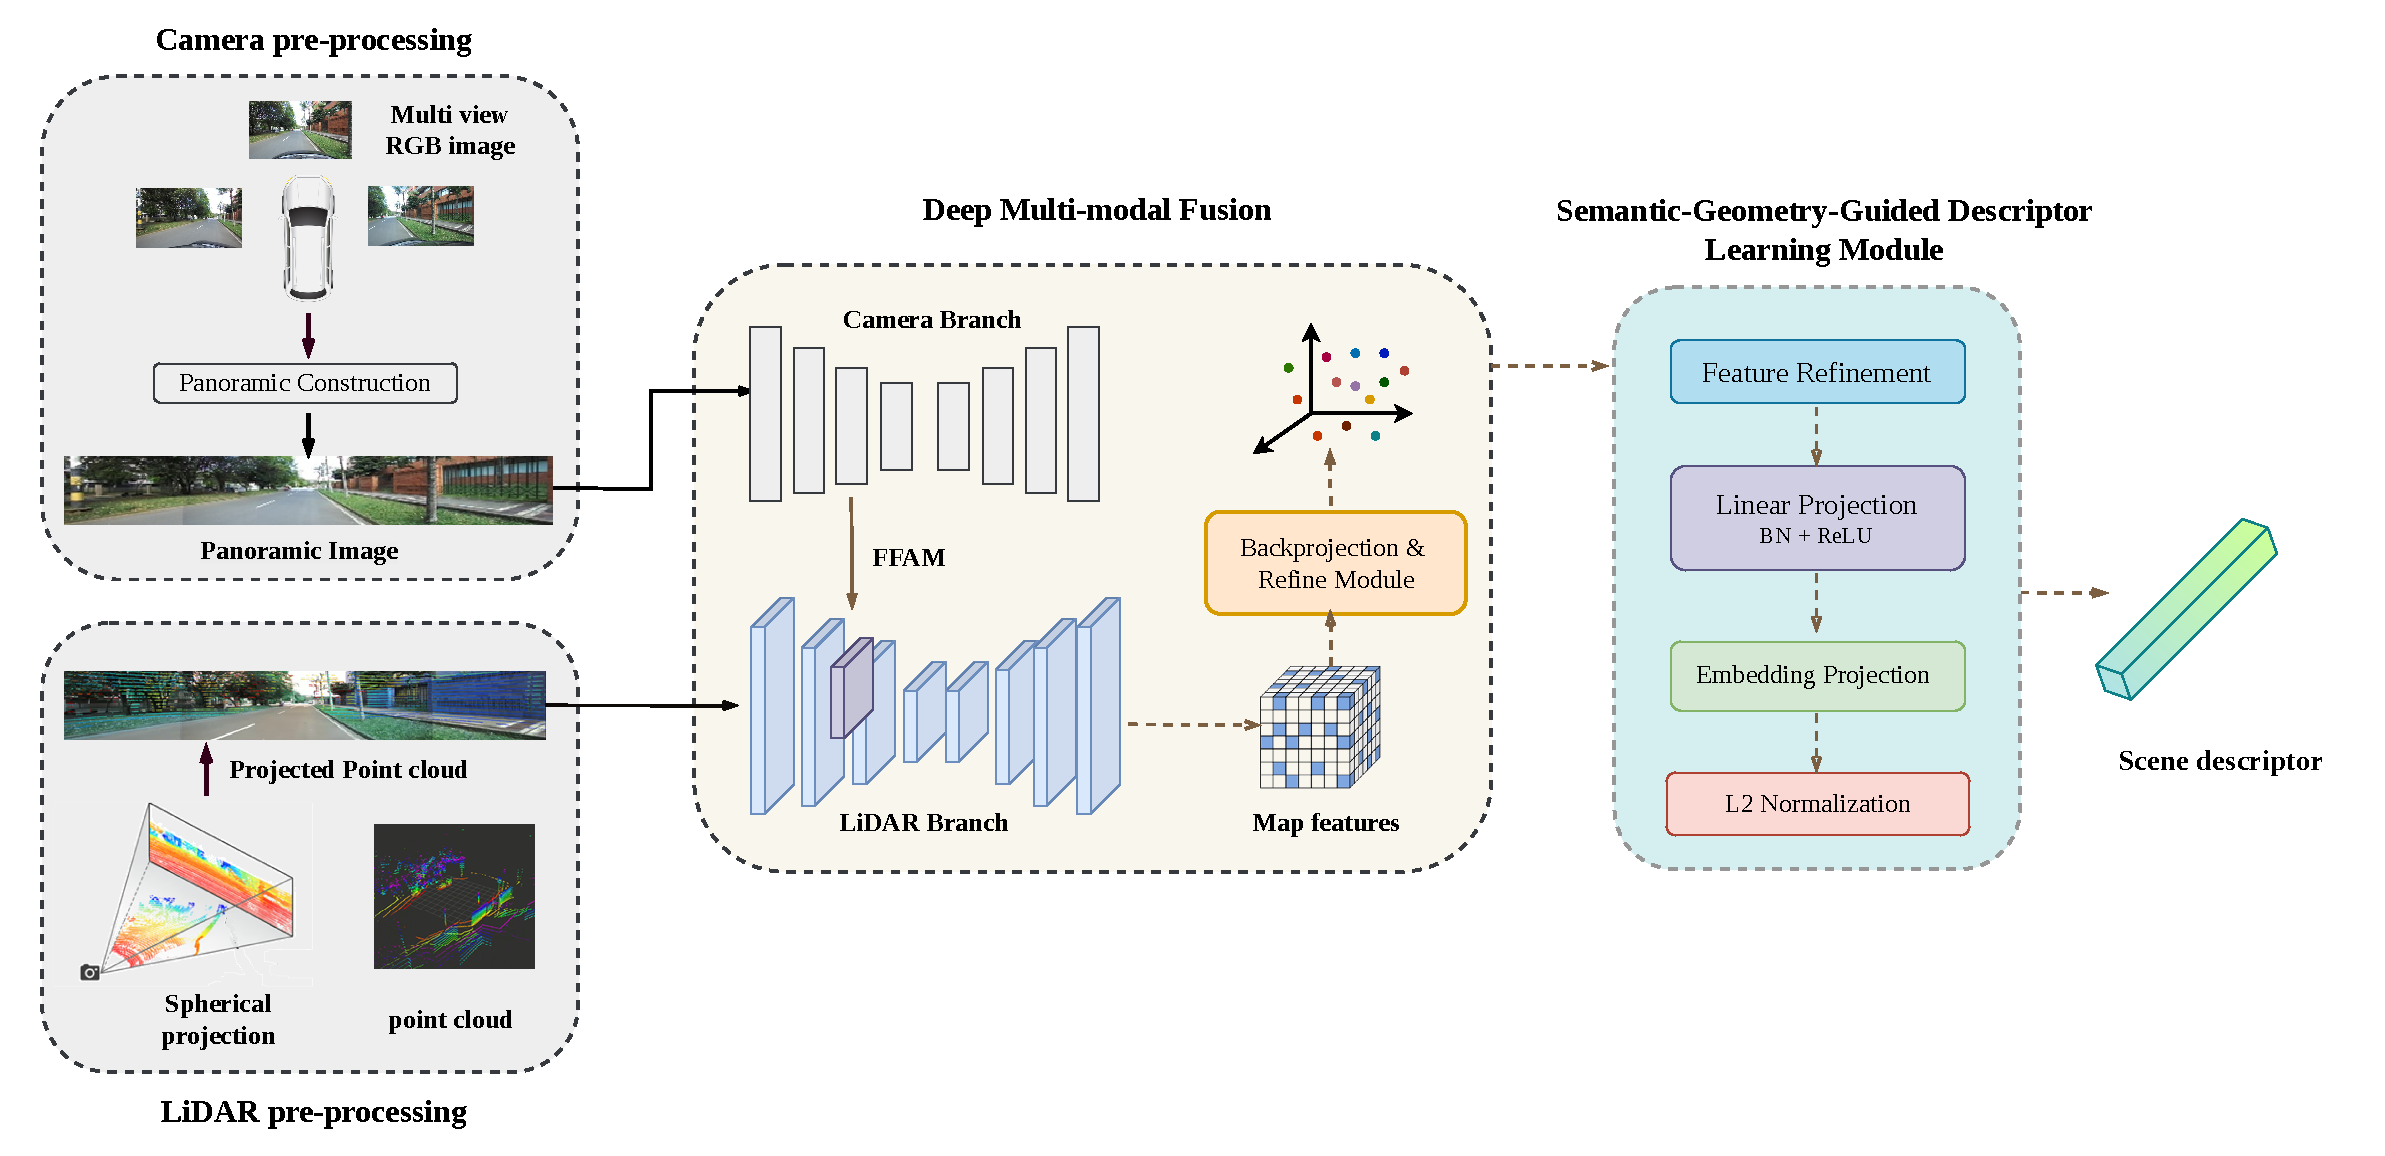
\includegraphics[width=\linewidth]{Figures/Pipeline-global-descriptor-multi-modal.pdf} 	
	\captionof{figure}{Main core of the proposed pipeline for generating global descriptors from multimodal data. The point cloud is projected onto the panoramic image, and both modalities are processed through a shared backbone to extract refined 3D features. A learnable global descriptor head aggregates these features into a compact embedding for place recognition.}	
	\label{fig:pipeline}
\end{strip}

Large-scale annotated datasets~\cite{behley2019semantickitti, nuscenes2019, SunKDCPTGZCCVHN20, eu_longterm_dataset} have highlighted the importance of semantic supervision for structured scene understanding; however, extracting semantically robust and globally discriminative representations from single modalities remains challenging.
These observations motivate multimodal fusion strategies that integrate LiDAR geometry with visual appearance. By leveraging the complementary nature of spatial structure and texture, multimodal approaches mitigate the modality-specific degradation factors that affect single-sensor systems. Nevertheless, multimodal fusion introduces additional challenges, including precise extrinsic calibration, accurate projection of 3D points onto the image plane, reliable cross-modal alignment, and increased computational complexity. \\

Motivated by the approach presented in~\cite{Snchez-Garca2025}, our pipeline as depicted in Fig~\ref{fig:pipeline} leverages panoramic images generated through a homography-based mosaicing of three stereo cameras, together with the corresponding LiDAR point cloud. The 3D measurements are projected onto the panoramic mosaic, effectively transforming geometric information into a 2D representation aligned with the image domain. In this manner, each pixel is enriched with geometric attributes associated with a spatial point prior to being processed by the semantic segmentation network. The output of the point cloud branch is subsequently re-projected into the 3D domain, following the strategy introduced in \cite{Lin2025},
In addition to semantic segmentation, we introduce a learnable global descriptor head that transforms refined 3D multimodal features into a compact and discriminative embedding suitable for place recognition. Unlike conventional approaches that rely on handcrafted pooling or intermediate logits, the proposed descriptor is extracted directly from the refined 3D feature space and aggregated through an attention-based global pooling mechanism. This design allows the network to selectively emphasize structurally stable and semantically informative regions while suppressing dynamic or less discriminative elements.

\begin{table*}[]
\caption{\scriptsize\MakeUppercase{Classical Handcrafted Local and Global Feature Descriptors for LiDAR Data}}
\label{tab:lidar-only-local-descriptors}
\begin{tabular}{|c|c|c|c|c|c|c|c|}
\hline
\rowcolor[HTML]{EFEFEF} 
\textbf{Ref.} & \textbf{Type} & \textbf{Descriptor} & \textbf{Main approach} & \textbf{\begin{tabular}[c]{@{}c@{}}Robust to\\ Viewpoint\end{tabular}} & \textbf{Semantic} & \textbf{Strengths} & \textbf{Limitation} \\ \hline
\multicolumn{1}{|c|}{\cite{Johnson1999}} &  & Handcrafted & \begin{tabular}[c]{@{}c@{}}Gradient-based keypoint \\ descriptor\end{tabular} & \begin{tabular}[c]{@{}c@{}}keypoint-\\ based\end{tabular} & X & \begin{tabular}[c]{@{}c@{}}Robust to illumination changes;\\  foundational for local matching\end{tabular} & \begin{tabular}[c]{@{}c@{}}Originally 2D; not designed \\ for raw 3D LiDAR; \\ computationally expensive\end{tabular} \\ \cline{1-1} \cline{3-8} 
\multicolumn{1}{|c|}{\cite{HungarConstanze2019}} &  & Handcrafted & \begin{tabular}[c]{@{}c@{}}Gradients of LiDAR intensity \\ for local description\end{tabular} & local frame & X & \begin{tabular}[c]{@{}c@{}}Exploits intensity information; \\ suitable for map-based localization\end{tabular} & \begin{tabular}[c]{@{}c@{}}Sensitive to intensity noise; \\ depends on sensor calibration\end{tabular} \\ \cline{1-1} \cline{3-8} 
\multicolumn{1}{|c|}{\cite{GuoJiadong2019}} &  & Handcrafted & \begin{tabular}[c]{@{}c@{}}Intensity distribution-based \\ descriptor\end{tabular} & Partial & X & \begin{tabular}[c]{@{}c@{}}Improves distinctiveness over \\ geometry-only descriptors\end{tabular} & \begin{tabular}[c]{@{}c@{}}Performance depends \\ on intensity consistency \\ across sessions\end{tabular} \\ \cline{1-1} \cline{3-8} 
\multicolumn{1}{|c|}{\cite{RusuRadu2009}} & \multirow{-4}{*}{Local} & \begin{tabular}[c]{@{}c@{}}Handcrafted \\ geometric\end{tabular} & \begin{tabular}[c]{@{}c@{}}Histogram of surface normals \\ and curvature relationships\end{tabular} & \begin{tabular}[c]{@{}c@{}}Local  \\ frame\end{tabular} & X & \begin{tabular}[c]{@{}c@{}}Fast; widely adopted; effective \\ for registration\end{tabular} & \begin{tabular}[c]{@{}c@{}}Sensitive to noise and \\ sparse point clouds; \\ limited discriminative power\end{tabular} \\ \hline
\multicolumn{1}{|c|}{\cite{Fan2021}} &  & Semantic & \begin{tabular}[c]{@{}c@{}}Histogram/topological structure \\ enriched with semantic classes\end{tabular} & $\checkmark$ & $\checkmark$ & \begin{tabular}[c]{@{}c@{}}Robust to structural \\ changes in urban scenes\end{tabular} & \begin{tabular}[c]{@{}c@{}}Depends on segmentation \\ accuracy\end{tabular} \\ \cline{1-1} \cline{3-8} 
\multicolumn{1}{|c|}{\cite{Liao2022}} &  & \begin{tabular}[c]{@{}c@{}}Topological-\\ semantic\end{tabular} & \begin{tabular}[c]{@{}c@{}}Graph-based topological \\ descriptor with semantic labels\end{tabular} & $\checkmark$ & $\checkmark$ & \begin{tabular}[c]{@{}c@{}}Robust to viewpoint variations; \\ interpretable structure\end{tabular} & \begin{tabular}[c]{@{}c@{}}Sensitive to semantic \\ misclassification\end{tabular} \\ \cline{1-1} \cline{3-8} 
\multicolumn{1}{|c|}{\cite{Cao2018}} &  & Geometric & \begin{tabular}[c]{@{}c@{}}Laser-based urban structural \\ descriptor\end{tabular} & $\checkmark$ & X & \begin{tabular}[c]{@{}c@{}}Effective in structured urban \\ environments\end{tabular} & \begin{tabular}[c]{@{}c@{}}Limited performance in \\ unstructured scenes\end{tabular} \\ \cline{1-1} \cline{3-8} 
\multicolumn{1}{|c|}{\cite{Wang2020}} &  & \begin{tabular}[c]{@{}c@{}}Projection-\\ based\end{tabular} & \begin{tabular}[c]{@{}c@{}}Polar image representation \\ (Iris-like encoding)\end{tabular} & $\checkmark$ & X & \begin{tabular}[c]{@{}c@{}}Rotation-invariant; compact \\ representation\end{tabular} & \begin{tabular}[c]{@{}c@{}}Sensitive to dynamic \\ changes\end{tabular} \\ \cline{1-1} \cline{3-8} 
\multicolumn{1}{|c|}{\cite{Fan2020}} &  & \begin{tabular}[c]{@{}c@{}}Segmentation-\\ based\end{tabular} & \begin{tabular}[c]{@{}c@{}}Egocentric segmentation-\\ driven structural descriptor\end{tabular} & $\checkmark$ & \begin{tabular}[c]{@{}c@{}}$\checkmark$ \\ partial\end{tabular} & \begin{tabular}[c]{@{}c@{}}Encodes structural context; \\ improved distinctiveness\end{tabular} & \begin{tabular}[c]{@{}c@{}}Dependent on reliable \\ segmentation\end{tabular} \\ \cline{1-1} \cline{3-8} 
\multicolumn{1}{|c|}{\cite{Li2021}} &  & Semantic & \begin{tabular}[c]{@{}c@{}}Extension of Scan Context \\ with semantic labels\end{tabular} & - & $\checkmark$ & \begin{tabular}[c]{@{}c@{}}High robustness to seasonal \\ and illumination changes; \\ efficient matching\end{tabular} & \begin{tabular}[c]{@{}c@{}}Increased complexity \\ compared  to Scan \\ Context\end{tabular} \\ \cline{1-1} \cline{3-8} 
\multicolumn{1}{|c|}{\cite{Xiang2021}} &  & \begin{tabular}[c]{@{}c@{}}Compact \\ geometric\end{tabular} & \begin{tabular}[c]{@{}c@{}}Compact 3D histogram-\\ based descriptor\end{tabular} & - & X & \begin{tabular}[c]{@{}c@{}}Very fast; suitable for indoor \\ mapping\end{tabular} & \begin{tabular}[c]{@{}c@{}}Lower discriminative power \\ in complex scenes\end{tabular} \\ \cline{1-1} \cline{3-8} 
\multicolumn{1}{|c|}{\cite{Zhou2022}} &  & Statistical & \begin{tabular}[c]{@{}c@{}}Normal distribution modeling \\ of geometric features\end{tabular} & $\checkmark$ & X & Compact and noise-robust & \begin{tabular}[c]{@{}c@{}}Sensitive to major \\ structural variations\end{tabular} \\ \cline{1-1} \cline{3-8} 
\multicolumn{1}{|c|}{\cite{Zhang2022}} &  & Geometric & \begin{tabular}[c]{@{}c@{}}Structural descriptor for \\ registration and LCD\end{tabular} & $\checkmark$ & X & \begin{tabular}[c]{@{}c@{}}Robust to occlusions; useful for \\ joint registration\end{tabular} & \begin{tabular}[c]{@{}c@{}}Moderate computational \\ cost\end{tabular} \\ \cline{1-1} \cline{3-8} 
\multicolumn{1}{|c|}{\cite{Wang2023}} &  & \begin{tabular}[c]{@{}c@{}}Projection-\\ based\end{tabular} & \begin{tabular}[c]{@{}c@{}}Double 3D-to-2D projection \\ strategy\end{tabular} & - & X & \begin{tabular}[c]{@{}c@{}}Higher discriminability than \\ single  projection methods\end{tabular} & \begin{tabular}[c]{@{}c@{}}Possible loss of fine 3D \\ information\end{tabular} \\ \cline{1-1} \cline{3-8} 
\multicolumn{1}{|c|}{\cite{Liu2023}} & \multirow{-11}{*}{Global} & Geometric & \begin{tabular}[c]{@{}c@{}}Enhanced Cartesian \\ histogram representation\end{tabular} & - & X & Lightweight; real-time capable & \begin{tabular}[c]{@{}c@{}}Sensitive to dynamic objects \\ and structural changes\end{tabular} \\ \hline
\end{tabular}
\end{table*}

To validate our framework, we conducted extensive experiments on the SemanticKITTI dataset, focusing on the object classes to be identified (vehicles, pedestrians, façades, and traffic signs). Our contributions are listed below: 

\begin{itemize}
    \item Building upon the VPA-Net architecture, we extend its multimodal fusion framework beyond dense semantic segmentation by introducing a learnable global descriptor head that extracts compact scene-level embeddings directly from refined 3D features.
    \item We integrate a homography-based panoramic mosaicing strategy to enlarge the field of view and strengthen multimodal spatial correspondence, enabling more context-aware feature learning.
    \item We unify dense semantic segmentation and global place-level representation within a single end-to-end trainable framework, bridging multimodal perception and scene retrieval without modifying the core backbone structure.
\end{itemize}

The remainder of this paper is structured as follows. Section II reviews the related work. Section III presents the details of our proposed network. Section IV discusses the experimental results. Conclusions and future work are drawn in the last section. 
	\section{Related Works}~\label{sec:related-works}

Research on 3D descriptors for place recognition and SLAM has evolved from classical handcrafted methods to learning-based and multi-modal fusion approaches. Early techniques relied on manually designed geometric features extracted from point clouds, either locally or globally, providing efficient but limited representations. More recently, deep learning methods operating solely on point clouds have demonstrated superior discriminative power by automatically learning invariant and task-optimized features. However, since LiDAR geometry alone may be insufficient in perceptually ambiguous or long-term changing environments, there is growing interest in learning descriptors from fused sensory information, particularly LiDAR–camera combinations, to exploit complementary geometric and visual cues. Motivated by this, this section reviews first the analyzes of classical geometric descriptors, then learning-based methods using only point clouds, and finally approaches based on LiDAR–camera fusion, highlighting the importance of multi-modal learned representations for robust long-term localization.

\subsection{LiDAR-Based Handcrafted Local and Global Descriptors}~\label{subsec:lidar-only-local-global-descriptors}

A LiDAR-based local descriptor is a compact representation extracted from the geometric neighborhood of a 3D point in a LiDAR point cloud. It encodes local spatial structure, shape distribution, and possibly reflectance information to facilitate correspondence estimation, feature matching, or higher-level scene understanding tasks.

Table~\ref{tab:lidar-only-local-descriptors} summarizes key handcrafted local and global descriptors for LiDAR point clouds, highlighting their approaches, invariance properties, strengths, and limitations. Handcrafted methods such as Spin Images \cite{Johnson1999} and LiDAR intensity-based descriptors \cite{HungarConstanze2019} rely on geometric and intensity gradients to capture local structure, offering robustness to illumination changes but often at high computational cost. Learning-based approaches like USIP \cite{Li2019} and PPF-AE \cite{deng2018} leverage unsupervised learning to identify stable keypoints and encode geometric relationships, providing improved repeatability and robustness but with increased complexity. Overall, while handcrafted descriptors laid the foundation for local feature extraction in 3D point clouds, learning-based methods have shown superior performance by automatically optimizing representations for specific tasks, albeit with trade-offs in computational efficiency.

While LiDAR-based global descriptor is a holistic representation computed from a full 3D LiDAR scan, encoding global geometric layout and structural patterns of the environment into a compact embedding suitable for place recognition and loop closure detection.

These descriptors range from geometric and projection-based methods to segmentation-driven approaches, each with unique advantages and challenges. For instance, semantic-enriched descriptors \cite{Fan2021, Liao2022} offer improved discriminability but depend heavily on accurate segmentation, while geometric descriptors \cite{Cao2018, Zhang2022} are effective in structured environments but may struggle in unstructured scenes. Projection-based methods \cite{Wang2020, Wang2023} provide compact representations but can lose fine 3D details. Overall, while these handcrafted global descriptors have been foundational in LiDAR-based place recognition and localization, they often face limitations in dynamic or changing environments, motivating the shift towards learning-based and multi-modal approaches for enhanced robustness.

%LiDAR-only semantic segmentation methods aim to assign a semantic label to each 3D point in a point cloud using exclusively geometric information captured by the sensor. These approaches rely on the spatial structure, depth measurements, an local geometric properties of the environment without incorporating visual texture cues from cameras. Broadly, LiDAR-based segmentation techniques can be categorized into classical geometric descriptors based on points cloud, voxel, image methods.  

%\subsubsection{Point cloud-based methods} \label{subsubsec:point-cloud-method}

%Early methods such as \cite{qi2017pointnetdeeplearningpoint} and \cite{qi2017pointnet++} employ Multi-Layer Perceptrons (MLPs) combined with KNN-based hierarchical grouping to learn local geometric structures from raw point sets. These approaches rely on hierarchical aggregation mechanisms to progressively capture neighborhood information. Similarly, \cite{qian2022pointnextrevisitingpointnetimproved} extends MLP-based hierarchical architectures by incorporating efficient MLP stacking and explicit KNN neighbor search to improve scalability and training stability.
%More advanced point-based convolutional models are introduced in \cite{thomas2024kpconvxmodernizingkernelpoint}, where kernel point convolution combined with attention mechanisms enhances local feature modeling. In \cite{hu2020randlanetefficientsemanticsegmentation}, attention is further integrated into point-based MLP networks with detection-aware optimization, incorporating random sampling and local feature aggregation strategies evaluated on SemanticKITTI. Additionally, \cite{yan20222dpass2dpriorsassisted} proposes a 3D point network enhanced through knowledge distillation from 2D priors, enabling semantic transfer from image-based representations into 3D space.
%Attention mechanisms and global context modeling become central in later works. The self-attention framework in \cite{lai2023sphericaltransformerlidarbased3d} adopts a transformer-style architecture operating on spherical-coordinate point representations, using radial window self-attention to capture global structural dependencies. In contrast, \cite{sanchez20253dlabelpropgeometricdrivendomaingeneralization} introduces a geometric label propagation strategy based on point alignment and ICP propagation, focusing on geometric optimization rather than end-to-end supervised learning.
%Transformer-based architectures dominate the most recent developments. Works \cite{zhao2021pointtransformer, NEURIPS2022_d78ece66, wu2024pointtransformerv3simpler} propose self-attention-driven models that operate directly on raw point sets. Specifically, [126] incorporates positional encoding into self-attention modules, [127] introduces efficient neighborhood attention with residual context blocks for end-to-end optimization, and [128] proposes a multi-scale global–local transformer fusion framework with computational optimizations to improve robustness in large-scale outdoor scenes.

%\subsubsection{Voxel-based methods} \label{subsubsec:voxel-based}

%\cite{Maturana2015} proposes a model architecture to address this problem by integrating a volumetric occupancy grid representation with a supervised 3D Convolutional Neural Network (3D CNN). Their approach guarantees invariance to rotation and resolution by employing fewer CNN parameters compared to other existing models, while still achieving reliable performance in object detection tasks.
%MinkLoc3D \cite{komorowski2020minkloc3dpointcloudbased} introduces a framework based on sparse 3D convolutions combined with a Feature Pyramid Network (FPN) backbone and GeM pooling to generate global descriptors. Similarity is computed using L2 distance between embeddings. MinkLoc3D-SI \cite{Zywanowski_2022} extends this approach by incorporating spherical coordinates and intensity information into the sparse convolution pipeline. It employs a triplet loss with explicit L2 distance between descriptors.
%EgoNN \cite{komorowski2021egonnegocentricneuralnetwork} leverages an FPN backbone enhanced with Efficient Channel Attention (ECA) modules to improve feature representation. It adopts global descriptor retrieval for place recognition, emphasizing improved contextual feature aggregation. Similarly, NDT-Transformer \cite{ZhouZhicheng2021} combines voxel-level statistical representations based on the Normal Distribution Transform (NDT) with transformer encoders to produce global descriptors,
%TransLoc3D \cite{xu2022transloc3dpointcloud} integrates NDT representations with an Adaptive Receptive Field Module (ARFM) and transformer architecture, followed by NetVLAD aggregation for global descriptor extraction. It uses triplet margin loss with L2 distance between descriptors, demonstrating robust performance on Oxford RobotCar. LCDNet \cite{cattaneo2022lcdnetdeeploopclosure} adopts a PV-RCNN backbone for feature extraction and employs NetVLAD for global descriptor aggregation, using L2 or cosine similarity metrics. It is evaluated on KITTI, KITTI-360, and Freiburg datasets.
%SVT-Net \cite{fan2021svtnetsuperlightweightsparse} introduces a Sparse Voxel Transformer (SVT) that captures both local and long-range structural dependencies before global descriptor retrieval, highlighting the importance of modeling extended spatial context. Finally, OverlapNetVLAD \cite{Fu2023ACP} employs a BEV-based feature extractor (BEVNet) combined with NetVLAD to produce descriptors typically compared via L2 distance, showing effectiveness on KITTI (2023).

%\subsubsection{Image-based methods} \label{subsubsec:image-based-methods}

%KPConv \cite{sanchez20253dlabelpropgeometricdrivendomaingeneralization} directly processes raw point clouds using Kernel Point Convolution, emphasizing geometric domain adaptation to improve generalization on SemanticKITTI. BEV-based convolutional fusion \cite{qiu2024pcbevefficientpolarcartesianbev} projects LiDAR data into polar and Cartesian Bird’s-Eye View representations and employs dual-branch CNNs with joint spatial–semantic optimization, evaluated on nuScenes.
%Hybrid approaches such as PointConv + SparseConv3D \cite{park2022pcscnetfast3dsemantic} operate on voxelized 3D grids, combining sparse 3D convolutions with point-based refinement in an end-to-end supervised framework. Harmonic Dense Convolution \cite{razani2021litehdseglidarsemanticsegmentation} also relies on voxel representations but introduces harmonic dense filters to improve computational efficiency. 
%Projection-based methods include 2D CNNs over spherical projections \cite{cortinhal2024salsanextfastuncertaintyawaresemantic}, which incorporate residual context and Bayesian uncertainty modeling, and 2D CNNs over polar range images \cite{nowruzi2021polarnetaccelerateddeepopen}, which apply standard supervised training on structured range-view representations.

\subsection{Learning-Based LiDAR Local and Global Descriptors}~\label{subsec:learning-based-local-global-descriptors}

Learning-based local descriptors are feature representations automatically learned from data using neural networks, encoding the geometric and/or semantic structure of local neighborhoods within a 2D or 3D space. This strategy is divide into 5 stages, as depicted in Table~\ref{tab:learning-based-lidar}: 1) point-based methods, which directly operate on raw point clouds; 2) voxel-based methods, which discretize the point cloud into a voxel grid and apply 3D convolutions; 3) segment-based methods, which extract local segments from the point cloud and learn descriptors based on their geometric and semantic properties; 4) projection-based methods, which project the 3D point cloud onto 2D planes; and 5) graph-based methods, which represent the point cloud as a graph structure and learn descriptors based on node and edge features.

Descriptor evolution across the references reflects increasing abstraction and contextual modeling. Early point-based descriptors such as PointNetVLAD~\cite{uy2018pointnetvladdeeppointcloud} and its extensions~\cite{liu2019lpdnet3dpointcloud, du2020dh3ddeephierarchical3d, HuiLe2021}, rely on NetVLAD aggregation for global feature pooling. 

\renewcommand{\arraystretch}{1.2}
\begin{table*}[!t]
\caption{\scriptsize\MakeUppercase{Learning-Based LiDAR Local and Global Descriptors}}
\label{tab:learning-based-lidar}
\centering
\begin{tabular}{|c|c|c|c|c|}
\hline
\rowcolor[HTML]{EFEFEF} 
\textbf{Ref.} & \textbf{Class} & \textbf{Descriptor} & \textbf{Feature} & \textbf{Similarity} \\ \hline
\cite{uy2018pointnetvladdeeppointcloud} &  & PointNet & NetVLAD & L2 / Cosine \\ \cline{1-1} \cline{3-5} 
\cite{liu2019lpdnet3dpointcloud} &  & GNN, DG-CNN & NetVLAD & Cosine \\ \cline{1-1} \cline{3-5} 
\cite{du2020dh3ddeephierarchical3d} &  & PointNet + FlexConv & NetVLAD, SE block & Cosine \\ \cline{1-1} \cline{3-5} 
\cite{HuiLe2021} &  & \begin{tabular}[c]{@{}c@{}}Pyramid Point \\ Transformer\end{tabular} & Pyramid VLAD & L2 / Cosine \\ \cline{1-1} \cline{3-5} 
\cite{Vidanapathirana_2022} & \multirow{-5}{*}{Point-based} & U-Net & ePN, 2nd-order pooling & L2 \\ \hline
\cite{komorowski2020minkloc3dpointcloudbased} &  & MinkLoc3D & Sparse 3D convolutions, FPN, GeM & L2 \\ \cline{1-1} \cline{3-5} 
\cite{Zywanowski_2022} &  & MinkLoc3D-SI & \begin{tabular}[c]{@{}c@{}}Sparse convolutions - spherical \\ coordinates - intensity; FPN; GeM\end{tabular} & L2 \\ \cline{1-1} \cline{3-5} 
\cite{komorowski2021egonnegocentricneuralnetwork} &  & EgoNN & FPN backbone; ECA attention & \begin{tabular}[c]{@{}c@{}}Uses global \\ descriptor retrieval\end{tabular} \\ \cline{1-1} \cline{3-5} 
\cite{ZhouZhicheng2021} &  & NDT-Transformer & \begin{tabular}[c]{@{}c@{}}Voxel-level statistical representation \\ (Normal Distribution Transform); \\ Transformer encoder;\end{tabular} & \begin{tabular}[c]{@{}c@{}}Uses descriptor \\ retrieval\end{tabular} \\ \cline{1-1} \cline{3-5} 
\cite{xu2022transloc3dpointcloud} & \multirow{-5}{*}{Voxel-based} & TransLoc3D & \begin{tabular}[c]{@{}c@{}}NDT representation; Adaptive \\ Receptive Field Module (ARFM); \\ Transformer; NetVLAD\end{tabular} & L2 \\ \hline
\cite{LiLin2021} &  & SA-LOAM & \begin{tabular}[c]{@{}c@{}}Edge and planar features (LOAM style); \\ spatial-appearance cues\end{tabular} & ICP-based \\ \cline{1-1} \cline{3-5} 
\cite{li2021sscsemanticscancontext} &  & SSC & \begin{tabular}[c]{@{}c@{}}PCA-based shape descriptors \\ from segmented point clouds\end{tabular} & \begin{tabular}[c]{@{}c@{}}L2 between \\ PCA descriptors\end{tabular} \\ \cline{1-1} \cline{3-5} 
\cite{fan2021semantic} &  & PCA-SSC & \begin{tabular}[c]{@{}c@{}}Improved PCA descriptors with \\ stronger geometric invariance\end{tabular} & L2 distance \\ \cline{1-1} \cline{3-5} 
\cite{yin2021psematchviewpointfreeplacerecognition} &  & PSE-Match & \begin{tabular}[c]{@{}c@{}}Probabilistic Shape Encoding \\ (mixture-model representation)\end{tabular} & \begin{tabular}[c]{@{}c@{}}Probability-based \\ similarity measure\end{tabular} \\ \cline{1-1} \cline{3-5} 
\cite{TaoSong2022} & \multirow{-5}{*}{Segment-based} & Song et al. & \begin{tabular}[c]{@{}c@{}}Hybrid descriptor combining geometry, \\ intensity, and local topology\end{tabular} & L2 or cosine \\ \hline
\cite{Barros_2022} &  & AttDLNet & \begin{tabular}[c]{@{}c@{}}Attention-based CNN encoder on projection \\ images; multi-scale feature extraction\end{tabular} & L2 \\ \cline{1-1} \cline{3-5} 
\cite{YinFuying2021} &  & SphereVLAD & \begin{tabular}[c]{@{}c@{}}Spherical projection + deep CNN features\\  + VLAD aggregation\end{tabular} & L2 / cosine distance \\ \cline{1-1} \cline{3-5} 
\cite{zhao2022spherevladattentionbasedsignalenhancedviewpoint} &  & SphereVLAD++ & \begin{tabular}[c]{@{}c@{}}Improved SphereVLAD with multi-scale \\ projections and enhanced CNN backbone\end{tabular} & L2 distance \\ \cline{1-1} \cline{3-5} 
\cite{lu2022deepringlearningrototranslationinvariant} &  & DeepRING & \begin{tabular}[c]{@{}c@{}}Circular (ring-based) LiDAR projection; \\ CNN encoder for rotation-equivariant features\end{tabular} & \begin{tabular}[c]{@{}c@{}}Correlation-based \\ similarity\end{tabular} \\ \cline{1-1} \cline{3-5} 
\cite{luo2023bevplacelearninglidarbasedplace} & \multirow{-5}{*}{Projection-based} & BEVPlace & \begin{tabular}[c]{@{}c@{}}Bird’s-eye-view (BEV) projection; CNN \\ encoder with BEV-specific geometric priors\end{tabular} & L2 distance \\ \hline
\cite{kong2020semanticgraphbasedplace} &  & SGPR & \begin{tabular}[c]{@{}c@{}}Builds semantic graphs from \\ segmented point clouds\end{tabular} & \begin{tabular}[c]{@{}c@{}}Graph matching using \\ structural similarity metrics\end{tabular} \\ \cline{1-1} \cline{3-5} 
\cite{Zhu2020GOSMatchGM} &  & GOS Match & \begin{tabular}[c]{@{}c@{}}Graph-of-semantics representation where \\ each node = semantic instance \\ and edges = geometric/topological relations\end{tabular} & \begin{tabular}[c]{@{}c@{}}Graph similarity scoring \\ with node - edge\end{tabular} \\ \cline{1-1} \cline{3-5} 
\cite{GongYansong2021} &  & Gong et al. & \begin{tabular}[c]{@{}c@{}}Two-tier representation: local spatial relation \\ graph + global spatial topology; \\ semantic and geometric cues\end{tabular} & \begin{tabular}[c]{@{}c@{}}Coarse-to-fine graph \\ matching;\end{tabular} \\ \cline{1-1} \cline{3-5} 
\cite{pramatarov2021a} &  & BoxGraph & \begin{tabular}[c]{@{}c@{}}Semantic bounding box graph generated from \\ object detectors; boxes as nodes, \\ box relations as edges\end{tabular} & \begin{tabular}[c]{@{}c@{}}Graph matching with \\ similarity metrics\end{tabular} \\ \cline{1-1} \cline{3-5} 
\cite{cui2021dscdeepscancontext} & \multirow{-5}{*}{Graph-based} & \begin{tabular}[c]{@{}c@{}}Deep Scan\\ Context\end{tabular} & \begin{tabular}[c]{@{}c@{}}Learned high-dimensional scan context descriptor; \\ pseudo-cylindrical projection + neural embedding\end{tabular} & L2 \\ \hline
\end{tabular}
\end{table*}
\renewcommand{\arraystretch}{1.2}

Sparse convolution-based descriptors like MinkLoc3D~\cite{komorowski2020minkloc3dpointcloudbased} and MinkLoc3D-SI \cite{Zywanowski_2022} introduce hierarchical 3D feature encoding. EgoNN \cite{komorowski2021egonnegocentricneuralnetwork} integrates attention mechanisms for enhanced global retrieval.
Voxel-based descriptors such as NDT-Transformer~\cite{ZhouZhicheng2021} and TransLoc3D~\cite{xu2022transloc3dpointcloud} employ statistical encodings and transformer architectures to capture long-range spatial dependencies.
Segment-based descriptors like SSC~\cite{li2021sscsemanticscancontext}, PCA-SSC~\cite{fan2021semantic}, and PSE-Match~\cite{yin2021psematchviewpointfreeplacerecognition} focus on geometric invariance and probabilistic similarity modeling. Song et al.~\cite{TaoSong2022} propose hybrid descriptors combining geometry, intensity, and topology.
Projection-based descriptors including ADLNet~\cite{Barros_2022}, SphereVLAD~\cite{YinFuying2021}, SphereVLAD++~\cite{zhao2022spherevladattentionbasedsignalenhancedviewpoint}, DeepRING~\cite{lu2022deepringlearningrototranslationinvariant}, and BEVPlace~\cite{luo2023bevplacelearninglidarbasedplace} utilize CNN encoders on structured projections, incorporating multi-scale aggregation and rotation-equivariant mechanisms.
Graph-based descriptors introduce a structural paradigm shift. SGPR~\cite{kong2020semanticgraphbasedplace} and GNN-based matching methods~\cite{Zhu2020GOSMatchGM} encode semantic graphs and perform graph similarity learning. Cong et al.~\cite{GongYansong2021} integrate two-branch networks combining local spatial relations and graph-level topology. Box-Graph~\cite{pramatarov2021a} and DGC Scan Context~\cite{cui2021dscdeepscancontext} further exploit structural descriptors and graph matching metrics for robust place recognition.
Overall, descriptor development evolves from global feature aggregation toward relational graph modeling and topology-aware embeddings. \\

Feature representations vary significantly across paradigms. Point-based works such as U-Net~\cite{Vidanapathirana_2022} and MinkLoc3D~\cite{komorowski2020minkloc3dpointcloudbased} leverage sparse 3D convolutions, second-order pooling, and geometric descriptors. These methods focus on hierarchical geometric encoding.
Voxel-based features in NDT-Transformer~\cite{ZhouZhicheng2021} rely on statistical distribution modeling (Normal Distribution Transform), while TransLoc3D~\cite{xu2022transloc3dpointcloud} introduces adaptive receptive field modules and NetVLAD aggregation for enhanced contextual capture.
Segment-based approaches such as SSC~\cite{li2021sscsemanticscancontext} and PCA-SSC~\cite{fan2021semantic} employ PCA-derived geometric features, whereas PSE-Match~\cite{yin2021psematchviewpointfreeplacerecognition} models shapes probabilistically. Song et al.~\cite{TaoSong2022} integrate hybrid feature combinations including geometry and intensity.
Projection-based methods like SphereVLAD~\cite{YinFuying2021}, DeepRING~\cite{lu2022deepringlearningrototranslationinvariant}, and BEVPlace~\cite{luo2023bevplacelearninglidarbasedplace} extract features via CNN backbones applied to spherical or BEV projections, often incorporating rotation invariance and multi-scale representations.
Graph-based features explicitly encode nodes (e.g., semantic objects, segments, scan contexts) and edges (spatial relationships, topological adjacency). SGPR~\cite{kong2020semanticgraphbasedplace} builds semantic graphs, while [59] and [60] incorporate attention mechanisms and relational reasoning. Box-Graph~\cite{pramatarov2021a} and DGC Scan Context~\cite{cui2021dscdeepscancontext} emphasize structural graph descriptors and pose-invariant relational encoding.
Thus, feature design increasingly transitions from local geometric encoding toward structured relational representations. \\

Similarity computation strategies reflect methodological differences across paradigms. Most deep descriptor-based approaches, including~\cite{uy2018pointnetvladdeeppointcloud, HuiLe2021, Vidanapathirana_2022, komorowski2020minkloc3dpointcloudbased, Zywanowski_2022, xu2022transloc3dpointcloud, li2021sscsemanticscancontext, fan2021semantic, TaoSong2022, Barros_2022,YinFuying2021, zhao2022spherevladattentionbasedsignalenhancedviewpoint, luo2023bevplacelearninglidarbasedplace, cui2021dscdeepscancontext}, rely on L2 or cosine similarity in embedding space for efficient large-scale retrieval.
NetVLAD-based methods~\cite{uy2018pointnetvladdeeppointcloud,du2020dh3ddeephierarchical3d}, primarily use cosine similarity. SSC-based methods~\cite{li2021sscsemanticscancontext, fan2021semantic}, use L2 distance on PCA-derived descriptors. PSE-Match~\cite{yin2021psematchviewpointfreeplacerecognition} employs a probabilistic similarity measure. SA-LOAM~\cite{TaoSong2022} is distinct in using ICP-based alignment.
DeepRING~\cite{lu2022deepringlearningrototranslationinvariant} introduces correlation-based similarity for rotation robustness. Voxel-based NDT-Transformer~\cite{ZhouZhicheng2021} emphasizes descriptor retrieval frameworks.
Graph-based approaches adopt more complex structural matching strategies. SGPR \cite{kong2020semanticgraphbasedplace} uses graph matching and structural similarity scoring. GNN-based matching~\cite{Zhu2020GOSMatchGM} integrates graph similarity learning with node and edge-level reasoning. Cong et al.~\cite{GongYansong2021} apply contrastive graph matching. Box-Graph~\cite{pramatarov2021a} and DGC Scan Context~\cite{cui2021dscdeepscancontext} employ graph similarity metrics and L2 distance over relational descriptors.
Overall, similarity computation evolves from simple metric comparisons toward structured graph matching and relational reasoning, trading computational simplicity for structural robustness.

\subsection{Camera-LiDAR fusion methods} \label{subsec:camera-lidar-methods}

\begin{table*}[!t]
\caption{\scriptsize\MakeUppercase{Camera-LiDAR-fusion descriptors}}
\label{tab:camera-lidar-fusion-descriptors}
\centering
\begin{tabular}{|c|c|c|c|c|c|}
\hline
\rowcolor[HTML]{EFEFEF} 
\textbf{Ref.} & \textbf{Descriptor Type} & \textbf{Primary task} & \textbf{Multi modal Strategy} & \textbf{Strengths} & \textbf{Limitation} \\ \hline
\cite{komorowski2021minkloclidarmonocularimage} &  &  & \begin{tabular}[c]{@{}c@{}}Late fusion of LiDAR + \\ image embeddings\end{tabular} & \begin{tabular}[c]{@{}c@{}}Combines geometric and visual cues; \\ strong generalization\end{tabular} & \begin{tabular}[c]{@{}c@{}}Requires synchronized L-C; \\ moderate computational cost\end{tabular} \\ \cline{1-1} \cline{4-6} 
\cite{pan2021coralcoloredstructuralrepresentation} &  &  & \begin{tabular}[c]{@{}c@{}}Colored structural + \\ visual fusion\end{tabular} & \begin{tabular}[c]{@{}c@{}}Integrates appearance and structure; \\ robust place recognition\end{tabular} & \begin{tabular}[c]{@{}c@{}}Slightly lower recall than top-\\ performing multimodal methods\end{tabular} \\ \cline{1-1} \cline{4-6} 
\cite{Xu2025} &  &  & \begin{tabular}[c]{@{}c@{}}Cross-modal alignment - \\ orientation voting\end{tabular} & \begin{tabular}[c]{@{}c@{}}Orientation robustness via voting; \\ cross-modal alignment\end{tabular} & \begin{tabular}[c]{@{}c@{}}Sensor calibration complexity; \\ computational overhead\end{tabular} \\ \cline{1-1} \cline{4-6} 
\cite{Zhou2023} &  &  & \begin{tabular}[c]{@{}c@{}}Multi-scale LiDAR–camera \\ attention fusion\end{tabular} & \begin{tabular}[c]{@{}c@{}}Captures geometric and appearance \\ cues; robust under viewpoint change\end{tabular} & \begin{tabular}[c]{@{}c@{}}Accurate cross-modal calibration; \\ attention increases computational cost\end{tabular} \\ \cline{1-1} \cline{4-6} 
\cite{LIANG2025408} & \multirow{-5}{*}{\begin{tabular}[c]{@{}c@{}}Global \\ multimodal \\ descriptor\end{tabular}} & \multirow{-5}{*}{\begin{tabular}[c]{@{}c@{}}Place \\ Recognition\end{tabular}} & \begin{tabular}[c]{@{}c@{}}Bi-directional attentional \\ fusion\end{tabular} & \begin{tabular}[c]{@{}c@{}}Attentional refinement; resilient \\ to ambiguous scenes\end{tabular} & \begin{tabular}[c]{@{}c@{}}Higher computational cost due \\ to attention mechanism\end{tabular} \\ \hline
\cite{Li2023} &  &  & \begin{tabular}[c]{@{}c@{}}Multi-modal driving \\ fusion (RGB + LiDAR)\end{tabular} & \begin{tabular}[c]{@{}c@{}}Accurate multimodal segmentation; \\ integrates camera + LiDAR\end{tabular} & \begin{tabular}[c]{@{}c@{}}Computationally heavy; dataset-\\ specific performance\end{tabular} \\ \cline{1-1} \cline{4-6} 
\cite{Zhang2023} &  &  & \begin{tabular}[c]{@{}c@{}}Cross-modal transformer \\ fusion (RGB-X)\end{tabular} & \begin{tabular}[c]{@{}c@{}}Strong cross-modal feature learning; \\ improved semantic accuracy\end{tabular} & \begin{tabular}[c]{@{}c@{}}Transformer complexity; \\ high GPU memory usage\end{tabular} \\ \cline{1-1} \cline{4-6} 
\cite{hou2022pointtovoxelknowledgedistillationlidar} &  & \multirow{-3}{*}{\begin{tabular}[c]{@{}c@{}}Semantic \\ Segmentation\end{tabular}} & \begin{tabular}[c]{@{}c@{}}LiDAR + teacher features \\ (cross-modal distillation)\end{tabular} & \begin{tabular}[c]{@{}c@{}}Unsupervised knowledge distillation; \\ improves LiDAR descriptors\end{tabular} & \begin{tabular}[c]{@{}c@{}}Dependent on teacher model; \\ added training complexity\end{tabular} \\ \cline{1-1} \cline{3-6} 
\cite{2023PatRe.13709299H} &  &  & \begin{tabular}[c]{@{}c@{}}Multi-modal semantic \\ adaptation\end{tabular} & \begin{tabular}[c]{@{}c@{}}Handles domain shift; adapts \\ features without supervision\end{tabular} & \begin{tabular}[c]{@{}c@{}}Limited semantic precision compared \\ to fully supervised methods\end{tabular} \\ \cline{1-1} \cline{4-6} 
\cite{Cao2024} &  & \multirow{-2}{*}{\begin{tabular}[c]{@{}c@{}}Unsupervised \\ Domain \\ Adaptation\end{tabular}} & \begin{tabular}[c]{@{}c@{}}Multi-modal prior-guided \\ cross-domain adaptation\end{tabular} & \begin{tabular}[c]{@{}c@{}}Leverages image priors to reduce \\ domain gap; improves target \\ generalization\end{tabular} & \begin{tabular}[c]{@{}c@{}}Relies on quality of pseudo-labels; \\ sensitive to domain discrepancy\end{tabular} \\ \cline{1-1} \cline{3-6} 
\cite{LuoYang2025} &  &  & \begin{tabular}[c]{@{}c@{}}Cross-modal semantic \\ attention\end{tabular} & \begin{tabular}[c]{@{}c@{}}Focused semantic fusion; \\ enhances point-level semantics\end{tabular} & \begin{tabular}[c]{@{}c@{}}Requires accurate alignment \\ between sensors\end{tabular} \\ \cline{1-1} \cline{4-6} 
\cite{Lin2025} &  &  & Vision assistance for LiDAR & \begin{tabular}[c]{@{}c@{}}Leverages visual context to \\ improve LiDAR features\end{tabular} & \begin{tabular}[c]{@{}c@{}}Needs dense camera coverage; \\ limited generalization if camera fails\end{tabular} \\ \cline{1-1} \cline{4-6} 
\cite{Snchez-Garca2025} &  &  & Range + image fusion & \begin{tabular}[c]{@{}c@{}}Real-time performance; \\ robust multimodal segmentation\end{tabular} & \begin{tabular}[c]{@{}c@{}}Requires synchronized RGB; \\ may struggle with sparse LiDAR\end{tabular} \\ \cline{1-1} \cline{4-6} 
\cite{Lamichhane2025} &  &  & \begin{tabular}[c]{@{}c@{}}Depth-aware transformer \\ fusion\end{tabular} & \begin{tabular}[c]{@{}c@{}}Attention-based multimodal \\ context; strong semantic consistency\end{tabular} & \begin{tabular}[c]{@{}c@{}}Transformer complexity; \\ high memory usage\end{tabular} \\ \cline{1-1} \cline{4-6} 
\cite{Zhang2025} &  &  & LiDAR + fisheye fusion & \begin{tabular}[c]{@{}c@{}}Wide field-of-view coverage; \\ captures rich context\end{tabular} & \begin{tabular}[c]{@{}c@{}}Needs fisheye camera; \\ calibration-sensitive\end{tabular} \\ \cline{1-1} \cline{4-6} 
\cite{Tan2024} &  &  & Efficient perception fusion & \begin{tabular}[c]{@{}c@{}}Efficient fusion; perception-\\ aware features\end{tabular} & \begin{tabular}[c]{@{}c@{}}Focused on efficiency, may trade \\ off accuracy in complex scenarios\end{tabular} \\ \cline{1-1} \cline{4-6} 
\cite{Ni2024Robust3S} &  &  & \begin{tabular}[c]{@{}c@{}}Collaborative multimodal \\ learning\end{tabular} & \begin{tabular}[c]{@{}c@{}}Robust semantic feature \\ learning across modalities\end{tabular} & \begin{tabular}[c]{@{}c@{}}Higher training complexity; \\ needs aligned multimodal data\end{tabular} \\ \cline{1-1} \cline{4-6} 
\cite{Duan2024} &  &  & \begin{tabular}[c]{@{}c@{}}Camera–LiDAR cross-attention \\ with fast neighbor aggregation\end{tabular} & \begin{tabular}[c]{@{}c@{}}Efficient local-global feature \\ interaction; enhanced boundary \\ precision\end{tabular} & \begin{tabular}[c]{@{}c@{}}Attention and neighbor aggregation \\ increase memory usage\end{tabular} \\ \cline{4-6} 
\cite{Zhao2024} &  &  & \begin{tabular}[c]{@{}c@{}}Early–mid LiDAR–image \\ feature fusion\end{tabular} & \begin{tabular}[c]{@{}c@{}}Improves discriminative power of \\ LiDAR features using visual cues\end{tabular} & \begin{tabular}[c]{@{}c@{}}Dependent on synchronized RGB; \\ performance drops under poor lighting\end{tabular} \\ \cline{1-1} \cline{4-6} 
\cite{Du2023} &  &  & \begin{tabular}[c]{@{}c@{}}Feature-level RGB–LiDAR \\ fusion with hierarchical encoder\end{tabular} & \begin{tabular}[c]{@{}c@{}}Enhanced small-object segmentation; \\ better contextual modeling\end{tabular} & \begin{tabular}[c]{@{}c@{}}Dataset-dependent tuning; moderate \\ computational overhead\end{tabular} \\ \cline{1-1} \cline{4-6} 
\cite{Maiti_2023_CVPR} &  &  & \begin{tabular}[c]{@{}c@{}}Transformer-based multimodal \\ fusion\end{tabular} & \begin{tabular}[c]{@{}c@{}}Strong long-range cross-modal int.; \\ improved semantic consistency\end{tabular} & \begin{tabular}[c]{@{}c@{}}High GPU memory consumption; \\ complex training\end{tabular} \\ \cline{1-1} \cline{4-6} 
\cite{Wang2024} &  &  & \begin{tabular}[c]{@{}c@{}}Unified multimodal encoder \\ (optical + auxiliary modalities)\end{tabular} & \begin{tabular}[c]{@{}c@{}}Cost-effective design; scalable \\ multimodal integration\end{tabular} & \begin{tabular}[c]{@{}c@{}}Designed for remote sensing; limited \\ direct transfer to autonomous driving\end{tabular} \\ \cline{1-1} \cline{4-6} 
\cite{Ma2024} &  & \multirow{-13}{*}{\begin{tabular}[c]{@{}c@{}}Semantic \\ Segmentation\end{tabular}} & \begin{tabular}[c]{@{}c@{}}Hierarchical transformer-based \\ multimodal fusion\end{tabular} & \begin{tabular}[c]{@{}c@{}}Multi-scale contextual modeling; \\ strong global reasoning\end{tabular} & \begin{tabular}[c]{@{}c@{}}Computationally intensive; \\ large training data requirement\end{tabular} \\ \cline{1-1} \cline{3-6} 
\cite{Lu2024} &  & \begin{tabular}[c]{@{}c@{}}Semantic Scene \\ Completion\end{tabular} & \begin{tabular}[c]{@{}c@{}}Continuous fusion in \\ voxelized 3D grid\end{tabular} & \begin{tabular}[c]{@{}c@{}}Dense 3D context modeling; \\ consistent volumetric representation\end{tabular} & \begin{tabular}[c]{@{}c@{}}High memory usage due to voxel.;\\  computationally heavy\end{tabular} \\ \cline{1-1} \cline{3-6} 
\cite{Zhao2022} & \multirow{-20}{*}{\begin{tabular}[c]{@{}c@{}}Semantic \\ feature \\ descriptor\end{tabular}} & \begin{tabular}[c]{@{}c@{}}3D Vehicle \\ Detection\end{tabular} & \begin{tabular}[c]{@{}c@{}}Semantic-guided camera–LiDAR \\ feature augmentation\end{tabular} & \begin{tabular}[c]{@{}c@{}}Enhances object-aware fusion; \\ improves detection robustness\end{tabular} & \begin{tabular}[c]{@{}c@{}}Reliable semantic supervision; \\ added training complexity\end{tabular} \\ \hline
\end{tabular}
\end{table*}

The following analysis examines recent multimodal descriptor approaches by organizing them according to descriptor type, primary task, fusion strategy, strengths, and limitations. By structuring the comparison column-wise, this discussion highlights the evolution from global multimodal embeddings for place recognition toward semantically rich feature representations for dense scene understanding, while also identifying common design trends, performance advantages, and practical challenges associated with multimodal perception systems.
The Table~\ref{tab:camera-lidar-fusion-descriptors} distinguishes between Global multimodal descriptors (\cite{komorowski2021minkloclidarmonocularimage}–\cite{LIANG2025408}) and Semantic feature descriptors (\cite{Snchez-Garca2025,Lin2025},\cite{Li2023}-\cite{Zhao2022}), reflecting two fundamentally different design objectives. Global multimodal descriptors are primarily designed for place recognition, where LiDAR and visual data are fused to generate compact embeddings suitable for large-scale retrieval. These approaches emphasize discriminative global representation, cross-modal consistency, and robustness to viewpoint or illumination changes. In contrast, semantic feature descriptors target dense scene understanding tasks such as semantic segmentation, domain adaptation, scene completion, and object detection. Rather than producing a single global vector, these methods learn structured, context-rich feature maps that enable fine-grained prediction. This categorization highlights the methodological shift from retrieval-oriented embeddings to dense multimodal perception frameworks.

The section of primary tasks is boarded from global localization to comprehensive scene interpretation. Works~\cite{komorowski2021minkloclidarmonocularimage}–\cite{LIANG2025408} focus on place recognition, aiming to achieve reliable loop closure detection through multimodal global embeddings. From \cite{Zhao2022} onward, the emphasis shifts toward semantic segmentation, where multimodal fusion enhances pixel- or point-level classification accuracy. Domain adaptation strategies (\cite{Cao2024}, \cite{LuoYang2025}) address distribution shifts between datasets, improving generalization. More advanced tasks include semantic scene completion (\cite{Lu2024}), which infers volumetric occupancy and semantics, and 3D vehicle detection (\cite{Zhao2022}), which strengthens object-level reasoning through feature augmentation. This progression illustrates increasing task complexity and a move from global matching toward dense and structured environment understanding.
The multimodal strategies vary in fusion depth and architectural sophistication. Early approaches (\cite{komorowski2021minkloclidarmonocularimage, Zhao2024}) rely on direct LiDAR–image feature concatenation, while others introduce cross-modal alignment and orientation voting mechanisms (\cite{Xu2025, hou2022pointtovoxelknowledgedistillationlidar, LuoYang2025}) to enforce feature consistency. Attention-based fusion models (\cite{LIANG2025408, Lamichhane2025, Duan2024}) selectively weight complementary modality cues, improving robustness in ambiguous scenes. Transformer-based frameworks (\cite{Zhang2023, Maiti_2023_CVPR, Ma2024}) capture long-range contextual dependencies across modalities, representing a significant architectural advancement. Domain adaptation techniques (\cite{Cao2024,LuoYang2025}) leverage pseudo-label guidance to reduce domain gaps. Task-specific fusion schemes, such as voxelized semantic grids (\cite{Lu2024}) or feature augmentation for detection (\cite{Zhao2022}), tailor multimodal integration to downstream objectives. Overall, there is a clear evolution from simple feature fusion to structured cross-attention and unified encoder architectures.
Across the references, multimodal approaches consistently demonstrate improved robustness and contextual understanding. Methods such as~\cite{komorowski2021minkloclidarmonocularimage} and~\cite{pan2021coralcoloredstructuralrepresentation} effectively integrate geometry and visual structure, enhancing recognition reliability. Cross-modal alignment techniques (\cite{Xu2025, hou2022pointtovoxelknowledgedistillationlidar}) improve orientation consistency and discriminative capacity. Attention-based and transformer-driven models (\cite{LIANG2025408,Zhang2023, Maiti_2023_CVPR,Ma2024}) provide stronger global reasoning and context modeling, leading to improved segmentation accuracy and semantic consistency. Domain adaptation frameworks (\cite{Cao2024,LuoYang2025}) enhance generalization to unseen environments. Scene completion (\cite{Lu2024}) and detection frameworks (\cite{Zhao2022}) benefit from enriched object-aware fusion. In general, multimodal learning leverages complementary sensor characteristics to increase accuracy, resilience, and scene comprehension.
Despite their advantages, these approaches introduce several practical constraints. Many methods (\cite{komorowski2021minkloclidarmonocularimage, Zhou2023, Tan2024}) require accurate LiDAR–camera calibration and synchronization, which may be difficult in real-world deployments. Transformer-based and attention-heavy architectures (\cite{Zhang2023, Maiti_2023_CVPR,Ma2024}) significantly increase computational cost and training complexity. Domain adaptation techniques (\cite{Cao2024,LuoYang2025}) depend on pseudo-label quality and may struggle with severe distribution shifts. Some systems require specialized hardware, such as fisheye cameras (\cite{Zhang2025}), limiting scalability. Additionally, multimodal models often demand large aligned datasets (\cite{Ni2024Robust3S, Zhao2022}) and may exhibit sensitivity to sensor degradation or adverse lighting conditions. Therefore, while multimodal fusion improves perception performance, it also raises challenges in efficiency, scalability, and deployment robustness. \\

In summary, prior work shows that multimodal fusion substantially improves robustness and contextual awareness in both place recognition and dense perception tasks. Nevertheless, many existing approaches either prioritize global retrieval over object-level discrimination or focus on dense prediction without explicitly learning compact and discriminative multimodal descriptors. Moreover, challenges related to efficient fusion, scalability, and generalization remain open. In this context, we propose a method centered on the generation of multimodal fused descriptors that, through learning-based strategies, enable more robust object discrimination and a deeper understanding of the surrounding environment.
    \section{Methodology}~\label{sec:methodology}

The methodology for generating descriptors from a learning process based on the fusion of images and point clouds is divided into several stages: The first stage corresponds to the adjustment or preprocessing of the point cloud so that it can be projected onto the panoramic image. Then, based on the model presented by \cite{Lin2025}, the point cloud and the images are fed into the network to obtain perceptual features from both modalities individually through feature fusion using attention-based models.
Next, the projected point cloud is transformed into the 3D space using sparse convolutions within a refinement module to optimize the segmentation produced by both modalities. Finally, a trainable global descriptor is constructed, which transforms the multimodal 3D features into a discriminative embedding for the identification of the objects present in the scene.

\subsection{Panoramic Images Generation}~\label{subsec:panoramic-image-generation}

For comprehensive scene understanding and environmental awareness, the use of panoramic images offers significant advantages over single-camera setups, particularly in outdoor and large-scale autonomous perception scenarios. The panoramic representation of our multi-sensor system provides a 180-degree field of view, enabling the system to capture in front of the vehicle spatial context of a scene in a single frame. 

\newpage

\begin{strip}
	\centering
	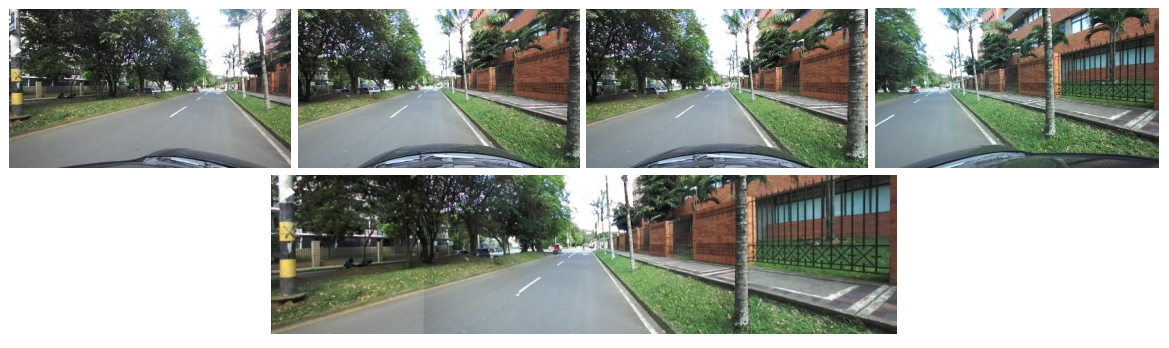
\includegraphics[width=\linewidth]{Figures/Stitching images_to_panoramic_uao.pdf} 	
	\captionof{figure}{Panoramic Image Generation via Multi-Camera Homography Alignment and Stitching.}	
	\label{fig:panoramic-image-generation}
\end{strip}

This holistic perception reduces blind spots and allows the model to reason about long-range spatial relationships between objects that would otherwise be distributed across multiple independent camera views. By observing the entire surrounding environment simultaneously, the system gains a more coherent representation of scene layout, object distribution, and structural continuity. \\
In contrast, single-camera images are inherently limited by their narrower field of view, which can restrict contextual reasoning and lead to partial observations of large structures such as buildings, intersections, or dynamic objects. This limitation may require additional multi-view fusion strategies to approximate a global understanding of the environment. Panoramic imagery, therefore, naturally supports richer contextual modeling, improved spatial completeness, and more consistent global representations of complex scenes.
The process begins with feature extraction, where salient keypoints and corresponding binary descriptors are detected using the ORB~\cite{Rublee2011} algorithm. ORB is selected due to its computational efficiency and robustness to rotation and illumination changes, making it suitable for real-time multi-camera applications. The input images have an initial spatial resolution of 1280 × 720 pixels, providing sufficient detail for reliable keypoint detection and matching.
Following feature extraction, a keypoint matching stage is performed between overlapping image pairs. Descriptor correspondences are established using a nearest-neighbor search strategy, typically based on Hamming distance due to ORB’s binary descriptors. These correspondences provide the geometric constraints necessary for estimating the transformation between views. \\

Next, a homography matrix is computed using the matched keypoints. To ensure robustness against incorrect correspondences (outliers), the homography is estimated using the RANSAC (Random Sample Consensus) algorithm. RANSAC iteratively selects minimal subsets of correspondences to compute candidate homographies and retains the solution that maximizes inlier consistency, thereby improving geometric accuracy.
Once the homography matrix is obtained, a perspective warping step is applied. One image is projected onto the coordinate frame of the reference image using a perspective transformation, aligning the overlapping regions into a common plane. This warping compensates for viewpoint differences between cameras under the planar scene assumption.
Finally, after geometric alignment and stitching, the resulting composite image undergoes cropping to remove redundant regions and boundary artifacts. The final panoramic output has a spatial resolution of 908 × 230 pixels, producing a compact, horizontally extended representation suitable for downstream perception tasks. This process is showed in Fig.~\ref{fig:panoramic-image-generation}.

\subsection{Preprocessing of the Point Cloud}~\label{subsec:lidar-preprocessing}

Several strategies can be employed to project 3D point clouds onto the image domain, including perspective, cylindrical~\cite{Kang2019RobustCP}, and spherical projections~\cite{HeYingshen2020}. The selection of the projection model is strongly influenced by the imaging geometry, sensor configuration, and especially the field of view of the camera system. In scenarios involving panoramic images with a wide angular coverage, spherical projection offers a more consistent geometric formulation than conventional perspective projection. Unlike perspective models, which are inherently limited to narrower fields of view and may introduce severe distortions at large viewing angles, spherical parameterization maintains the angular continuity of the scene by directly mapping LiDAR points according to their azimuth and elevation angles. This property ensures a more uniform spatial correspondence between 3D points and image pixels, thereby improving the stability of cross-modal alignment and facilitating more reliable multimodal feature fusion.
To perform the spherical projection as depicted in Fig.~\ref{fig:spherical-projection}, we first convert the Cartesian coordinates of the LiDAR points into spherical coordinates. Each point in the point cloud is represented by its range $r$, azimuth angle $\theta$, and elevation angle $\phi$. These type of images are dependent on the LiDAR's design parameters. It is important to know the vertical field of view (FOV) and the number of channels of the LiDAR to determine the resolution of the projected image. The vertical FOV defines the range of elevation angles that the LiDAR can capture, while the number of channels determines how many discrete elevation angles are sampled within that FOV. 

\newpage

\begin{strip}
	\centering
	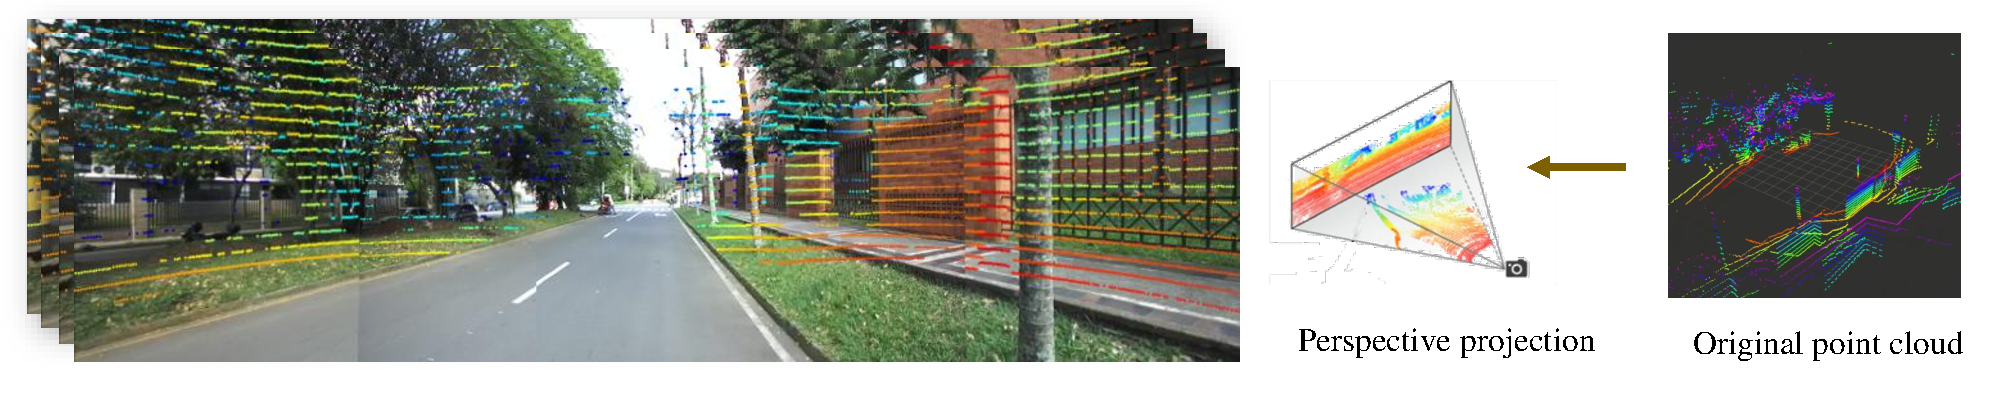
\includegraphics[width=\linewidth]{Figures/Spherical_point_cloud_projection.pdf} 	
	\captionof{figure}{Spherical Projection of LiDAR Point Cloud onto the Panoramic Image Plane.}	
	\label{fig:spherical-projection}
\end{strip}

This means that each channel corresponds to a specific elevation angle, and the point cloud can be projected onto a 2D image where each pixel corresponds to a specific azimuth and elevation angle. The horizontal resolution is determined by the azimuthal sampling, which is typically uniform across the 360-degree horizontal field of view. 
We compurte the depth of each point in the point cloud as the Euclidean distance from the LiDAR sensor to the point, which can be calculated using the formula:
\begin{equation}
    r = \sqrt{x^2 + y^2 + z^2}  
\end{equation}
where $x$, $y$, and $z$ are the Cartesian coordinates of the point.
Then, we calculate the azimuth angle $\theta$ and elevation angle $\phi$ for each point using the following formulas:
\begin{equation}
    \phi = \tan^{-1}\left(\frac{y}{x} \right) 
\end{equation}
\begin{equation}    \theta = \sin^{-1}\left(\frac{z}{r}\right)
\end{equation}
Afterward, each of the angles needs to be normalized to range between $[0,1]$, and then remapped to the perspective ranges of $[0, W]$ for yaw and $[0, H]$ for pitch, where $W$ and $H$ are the width and height of the projected image, respectively. The remapping can be performed using the following equations:

\begin{equation}    
    u = 0.5 \cdot \frac{\phi}{\pi} \cdot W
\end{equation}
\begin{equation}    
    v = \left(1.0 - \left( \frac{\theta + |fov_{down}|}{fov} \right) \right)\cdot H
\end{equation}
where $fov$ is the total vertical field of view of the LiDAR, and $fov_{down}$ is the downward vertical field of view. The resulting coordinates $(u, v)$ represent the pixel location in the projected image corresponding to each point in the point cloud. This process effectively transforms the 3D spatial information from the LiDAR into a 2D representation that can be easily fused with the panoramic image data for subsequent feature extraction and descriptor generation.

\subsection{Deep Multi-Modal Semantic Segmentation}~\label{subsec:multi-modal-semantic-segmentation}
	%********************************************************************************
\section{Experiments and Results} \label{sec:results}
%********************************************************************************

This section describes the results obtained based on different experiments.

%----------------------------------------------------
\subsection{Dataset}~\label{subsec:dataset}
%----------------------------------------------------

In this study, we selected the SemanticKITTI dataset, a large scale vehicular scene point cloud dataset, for our experimental analysis. This dataset is a large-scale benckmark desgined for semantic scene understanding using LiDAR data in urban driving environments. It is built upon the raw point cloud sequences of the KITTI Vision Benchmark Suite and provides dense point-wise semantic annotation for all LiDAR scans in the odometry sequences. The dataset contains 19,130 frames for training, 4071 frames for validity, and 24,892 frames for testing. We treated train–valid–test sequences and 19 categories which are consistent with the benchmark algorithms. 
The dataset includes road, building, vegetation, car, pedestrian, bycicle, and traffic-related structures. In addition, it also provides precise vehicle poses, enabling the study of temporal consistency localization, and mapping tasks. \\

A key characteristic of SemanticKITTI is that the point clouds are typically represented in a range-view projection, where the 3D LiDAR measurements are mapped onto a 2D cylindrical image according to the sensor’s azimuth and elevation angles. This representation preserves the structured acquisition pattern of rotating LiDAR sensors and allows the use of convolutional neural networks originally developed for image processing. Many state-of-the-art semantic segmentation approaches operate in this representation before optionally projecting the predictions back to the 3D space. \\

In the context of this work, SemanticKITTI serves as the primary benchmark for evaluating the proposed global descriptor generation framework for urban environment. The dataset provides both the geometric structure pf large-scale urban scenes and the semantic information required to build semantically-aware descriptors. Specifically, the LiDAR scans are processed through a multi-modal perception pipeline where fused features derived from LiDAR and camera observations are used to generate semantic feature maps. These features are then back-projected to the 3D space and refined to produce a semantic point cloud representation, from which compact global descriptors are extracted.

%------------------------------------------------------------------------------
\subsection{Implementation Details}~\label{subsec:implementation-details}
%------------------------------------------------------------------------------
For the experiments on the Semantic KITTI dataset, we used a machine equipped with Intel i9-14900K CPU and an NVIDIA GeForce RTX TITAN 24GB GPU. We implemented the proposed method in PyTorch~\cite{paszke2019pytorchimperativestylehighperformance},using ResNet-34~\cite{he2015deepresiduallearningimage} and SalsaNext~\cite{cortinhal2024salsanextfastuncertaintyawaresemantic} as the backbones for the camera stream and LiDAR stream, respectively. The parameters of ResNet-34 were initialized with a pretrained ImageNet model \cite{deng2009imagenet}. The network was trained for 20 epochs. \\

The training process starts with an initial learning rate of 0.001, which is progressively adapted during optimization using a warmup-cosine scheduling strategy. This approach combines an inicial warmup phase with a cosine annealing decay, allowing the learning rate to increase gradually at the beginning of training and then decrease smoothly as training progresses.
During the warmup stage, the learning rate is linearly increased from a very small value to the target learning rate. This phase lasts for a predefined number of iterations determined by:
\begin{equation}
    N_{warmup} = E_{warmup} \times |D_{train}|
\end{equation}
where $E_{warmup}$ represents the number of warmup epochs and $|D_{train}|$ corresponds to the number of mini-batches in the training dataloader. After the warmup period, the learning rate follows a cosine annealing schedule, which gtadually reduces the learning rate according to:
\begin{equation}
    \eta_t = \eta_0 \cdot \frac{1}{2} \left (1 + \cos \left (\frac{\pi t}{T_{max}} \right ) \right )
\end{equation}
The batch size was set to 4 for training stage and 2 for validation stage. To prevent overfitting, we employed various data augmentation strategies, including random horizontal flipping, color jittering, 2-D random rotation, and random cropping.

	\section{Conclusions} \label{sec:conclusion}
This work presented a two-stage multimodal framework that connects semantic perception with global candidate retrieval. The staged optimization and evaluator-specific reporting distinguish range-view segmentation, native point-level refinement, and external 3D audit results. The segmentation stage preserves useful evidence from persistent and landmark classes, but neither the complete multimodal FFAM++ configuration nor refinement establishes an overall mIoU advantage over the strongest segmentation baselines. Because RGB and FFAM++ are introduced together in the available comparison, the specific contribution of the additional channel gate remains unquantified.

SGMD is not intended to recognize absolute locations or make final loop-closure decisions. On the unseen SemanticKITTI sequence 08, temporal submaps improve spatial Recall@K over individual frames. However, Scan Context and M2DP remain substantially stronger at strict spatial thresholds. SGMD instead produces rankings with high semantic and landmark agreement. Landmark-aware re-ranking increases this agreement and improves strict 5\,m and 10\,m Recall@20 on sequence 08, although the gain is not consistent at the relaxed 20\,m threshold.

The supported contribution is therefore a semantic candidate-retrieval representation that preserves scene composition and persistent landmark evidence. Its role is complementary to geometry-based descriptors rather than a replacement for strict spatial retrieval. Evaluation on cross-session data with seasonal, illumination, or structural changes remains necessary before claiming long-term place-recognition robustness.

	\printbibliography
    %%-------------------------------------------------------------------------------------------------------------------------------------
%                                                   BIOGRAPHY
%-------------------------------------------------------------------------------------------------------------------------------------
\vspace{2.0cm}
\begin{IEEEbiography}[{
\includegraphics[width=1in,height=1.25in,clip,keepaspectratio]{Figures/Photo_AANP.png}}]{Alvaro Navarro-Perez}
    (Member, IEEE) received the B.Sc. degree in Electronic Engineering from the Universidad del Quindío, Colombia, in 2008, and the M.Sc. degree in Robotics and Automation from TU Dortmund University, Germany, in 2015. He is currently pursuing the Ph.D. degree in Engineering at the Universidad del Valle, Colombia.
    He is an Assistant Professor with the Faculty of Engineering, Universidad del Quindío. He is also a member of the IEEE Robotics and Automation Society (RAS) and the Technological Development Research Group (GIDET). His research interests include instrumentation systems, autonomous robots and localization and mapping for self-driving cars. His current research focuses on semantic mapping for long-term localization using multi-modal systems.
\end{IEEEbiography}
\vspace{-2.0cm}
\begin{IEEEbiography}[{
\includegraphics[width=1in,height=1.25in,clip,keepaspectratio]{Figures/Photo_BBC.jpg}}]{Bladimir Bacca-Cortes}
    received the degree in electronic engineering and the master’s degree in automation from the Universidad del Valle, Valle del Cauca, Cali, Colombia, in 1999 and 2004, respectively, and the Ph.D. degree in technology from the Universitat de Girona, Cataluña, Girona, Spain, in 2012. He is currently a Full Professor with the School of Electrical and Electronic Engineering, Universidad del  Valle. He is a member of the research group on Perception and Intelligent Systems. His research interests include mobile robotics, simultaneous localization and mapping systems, and computer vision
\end{IEEEbiography}
\vspace{-2.0cm}
\begin{IEEEbiography}[{
\includegraphics[width=1in,height=1.25in,clip,keepaspectratio]{Figures/Photo_ECB.jpg}}]{Eduardo Caicedo-Bravo}
    received the degree in electronic engineering and the master’s degree in automation from the Universidad del Valle, Valle del Cauca, Cali, Colombia, in 1985 and 1993, respectively, and the Ph.D. degree in Engineering from the Polytechnic University of Madrid-Spain in 1996. He is currently a Full Professor with the School of Electrical and Electronic Engineering, Universidad del  Valle. He is the director of the research group on Perception and Intelligent Systems (PSI). Author of several books and scientific articles, guest speaker at national and international events and visiting professor at international universities. He has worked projects with COLCIENCIAS, The European Union, CYTED, the Swiss Confederation and national companies. Areas of Interest: Smart Grids, Instrumentation Electronics, Intelligent Systems, Computational Intelligence and Robotics.
\end{IEEEbiography}
    
\end{document}
